\chapter{Μαθηματικά Εργαλεία}

Στο κεφάλαιο αυτό γίνεται εισαγωγή των μαθηματικών εργαλείων και βασικών εννοιών στα οποία βασίζεται η διπλωματική εργασία. Σκοπός του κεφαλαίου είναι η συμφιλίωση του αναγνώστη με αυτές τις έννοιες, έτσι ώστε να γίνει ομαλή η μετάβαση στα αποτελέσματα της διπλωματικής εργασίας στα κεφάλαια που ακολουθούν. 

Συνοπτικά, τρία είναι τα εργαλεία που θα παρουσιαστούν. Αρχικά θα γίνει μια εισαγωγή στα νευρωνικά δίκτυα RBF με έμφαση στην αρχιτεκτονική τους, στον τρόπο που χρησιμοποιούνται στις εφαρμογές αναγνώρισης και ελέγχου, καθώς και τις προσεγγιστικές τους ιδιότητες. Στην συνέχεια θα παρουσιαστεί ο Έλεγχος Προδιαγεγραμμένης Απόκρισης, ο σκοπός που χρησιμοποιείται σε αυτή την εργασία καθώς και επιχειρήματα που αποδεικνύουν την εγκυρότητα του, τόσο σε μαθηματικό επίπεδο όσο και με την χρήση προσομοιώσεων. Τέλος, θα γίνει μια συνοπτική εισαγωγή στην αρχιτεκτονική του υποσυστήματος που παράγει τα σήματα αναφοράς του σχήματος, καθώς και ποιοι είναι οι λόγοι που χρησιμοποιείται αυτή η μεθοδολογία και όχι κάποια άλλη.


%Artificial neural networks (ANNs) or connectionist systems are computing systems vaguely inspired by the biological neural networks that constitute animal brains.[1] Such systems "learn" (i.e. progressively improve performance on) tasks by considering examples, generally without task-specific programming. For example, in image recognition, they might learn to identify images that contain cats by analyzing example images that have been manually labeled as "cat" or "no cat" and using the results to identify cats in other images. They do this without any a priori knowledge about cats, e.g., that they have fur, tails, whiskers and cat-like faces. Instead, they evolve their own set of relevant characteristics from the learning material that they process.

\section{Νευρωνικά Δίκτυα RBF}
Με τον όρο \textit{Tεχνητά Νευρωνικά Δίκτυα} (Artificial Neural Networks) αναφερόμαστε σε μια κατηγορία μαθηματικών μοντέλων τα οποία προέκυψαν την δεκαετία του 1940 και είναι εμπνευσμένα από τα βιολογικά νευρωνικά δίκτυα τα οποία απαντώνται στους εγκεφάλους των ανθρώπων και των ζώων. Το κύριο χαρακτηριστικό των νευρωνικών δικτύων είναι η εγγενής ικανότητα μάθησης. Ως μάθηση μπορεί να οριστεί η σταδιακή βελτίωση της ικανότητας του δικτύου να επιλύει κάποιο πρόβλημα (π.χ. η σταδιακή προσέγγιση μίας συνάρτησης). Η μάθηση επιτυγχάνεται μέσω της εκπαίδευσης, μίας επαναληπτικής διαδικασίας σταδιακής προσαρμογής των παραμέτρων του δικτύου σε τιμές κατάλληλες ώστε να επιλύεται με επαρκή επιτυχία το προς εξέταση πρόβλημα.


Υπάρχουν πολλές κατηγορίες νευρωνικών δικτύων όπως τα Συνελικτικά Νευρωνικά Δίκτυα (Convolutional Neural Networks), τα Αναδρομικά Νευρωνικά Δίκτυα (Recurrent Neural Networks), τα Ακτινικά Νευρωνικά Δίκτυα (Radial Basis Networks), τα Πιθανοτικά Νευρωνικά Δίκτυα (Probabilistic Neural Networks) και άλλα, κάθε ένα κατάλληλο για διαφορετικό τύπο εφαρμογών. Εμείς θα χρησιμοποιήσουμε τα ακτινικά νευρωνικά δίκτυα τα οποία από εδώ και στο εξής θα αναφέρουμε ως \textit{δίκτυα RBF} καθώς είναι τα καταλληλότερα για προσέγγιση συναρτήσεων.

\subsection{Αρχιτεκτονική}
Η αρχιτεκτονική ενός RBF νευρωνικού δικτύου παρουσιάζεται στο σχήμα $(\ref{fig:rbf_network_architecture})$. Ένα RBF νευρωνικό δίκτυο αποτελείται από τρία επίπεδα, το επίπεδο εισόδου, το ενδιάμεσο ή κρυφό επίπεδο, και το επίπεδο εξόδου.

\begin{figure}
	\centering
	\documentclass{standalone}
\usepackage{tikz}
\usetikzlibrary{shapes,positioning,matrix}

\begin{document}
	%\begin{figure}[htp]
	%	\centering
		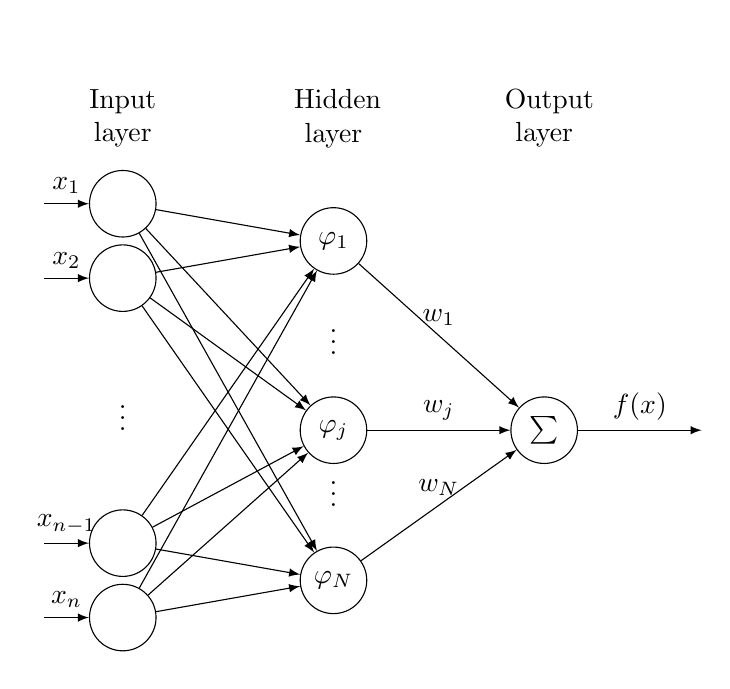
\begin{tikzpicture}[
		plain/.style={
			draw=none,
			fill=none,
		},
		net/.style={
			matrix of nodes,
			nodes={
				draw,
				circle,
				inner sep=8.5pt
			},
			nodes in empty cells,
			column sep=0.6cm,
			row sep=-11pt
		},
		>=latex
		]
		\matrix[net] (mat)
		{
			|[plain]| \parbox{1cm}{\centering Input\\layer} & 
			|[plain]| \parbox{1cm}{\centering Hidden\\layer} &
			|[plain]| \parbox{1cm}{\centering Output\\layer} \\
			& |[plain]| \\
			|[plain]| & \\
			& |[plain]| \\
			|[plain]| & |[plain]| $\vdots$\\
			|[plain]|$\vdots$& & \\
			|[plain]| & |[plain]|$\vdots$ \\
			& |[plain]| \\
			|[plain]| & \\
			& |[plain]| \\
		};
		
		
		\foreach \ai [count=\mi ]in {2,4}
		\draw[<-] (mat-\ai-1) -- node[above] {$x_\mi$} +(-1cm,0);
		\draw[<-] (mat-8-1) -- node[above] {$x_{n-1}$} +(-1cm,0);
		\draw[<-] (mat-10-1) -- node[above] {$x_{n}$} +(-1cm,0);
		
		\foreach \ai in {2,4,8,10}
		{\foreach \aii in {3,6,9}
			\draw[->] (mat-\ai-1) -- (mat-\aii-2);
		}
		
		% Final Weights
		\draw[->] (mat-3-2) --node[above]{$w_1$} (mat-6-3);
		\draw[->] (mat-6-2) --node[above]{$w_j$} (mat-6-3);
		\draw[->] (mat-9-2) --node[above]{$w_N$} (mat-6-3);
		\draw[->] (mat-6-3) -- node[above] {$f(x)$} +(2cm,0);
		
		\draw [] (mat-3-2) node(){$\varphi_1$};
		\draw [] (mat-6-2) node(){$\varphi_j$};
		\draw [] (mat-9-2) node(){$\varphi_N$};
		\draw [] (mat-6-3) node(){$\sum$};
		
		\end{tikzpicture}
		
\end{document}
	\caption{ Αρχιτεκτονική Νευρωνικού Δικτύου RBF }
	\label{fig:rbf_network_architecture}
\end{figure}

\textbf{Επίπεδο Εισόδου}: Η είσοδος ενός δικτύου RBF είναι ένα διάνυσμα $x = \begin{bmatrix} x_1,x_2, ..., x_n \end{bmatrix}^T$. Στα νευρωνικά δίκυτα αυτής της κατηγορίας το επίπεδο εισόδου είναι υπεύθυνο για την μετάδοση των επιμέρους ορισμάτων $x_i$ σε κάθε νευρώνα και όχι για κάποια περαιτέρω προεπεξεργασία δεδομένων.

\textbf{Κρυφό Επίπεδο:} Στο κρυφό επίπεδο λαμβάνει χώρο ο υπολογισμός των συναρτήσεων $\varphi_i(x)$ οι οποίες ονομάζονται \textit{συναρτήσεις βάσης} ή \textit{συναρτήσεις ενεργοποίησης}. Σε άλλους τύπους δικτύων μπορεί να υπάρχουν πάνω από ένα κρυφά επίπεδα, αλλά στα RBF δίκτυα που μελετάμε υπάρχει μόνο ένα.

Κάθε συνάρτηση βάσης είναι μια πραγματική συνάρτηση $\varphi: \mathbb{R}^n \rightarrow \mathbb{R} $, και αντιστοιχεί σε ένα σημείο του χώρου $c \in \mathbb{R}^n$. Οι συναρτήσεις $\varphi$ είναι ακτινικές συναρτήσεις, που σημαίνει πως αποτέλεσμα τους εξαρτάται από την απόσταση της εισόδου $x$ από το σημείο $c$, ή αλλιώς μαθηματικά:
\begin{equation*}
	\varphi(x,c) = \varphi(\| x - c \|)
\end{equation*}
και από εκεί προκύπτει και η ονομασία Ακτινικά Νευρωνικά Δίκτυα. Τυπικές ακτινικές συναρτήσεις είναι η γκαουσιανή, η τετραγωνική, η αντίστροφη τετραγωνική και άλλες~\cite{wiki:rbf}, ωστόσο σε αυτήν την εργασία θα χρησιμοποιήσουμε τις γκαουσιανές συναρτήσεις οι οποίες έχουν την μορφή
\begin{equation*}
	\varphi(x) = \exp \left( - \left\| \frac{x - c}{\sigma}\right\|^2 \right)
\end{equation*}
Το σημείο $c$ ονομάζεται \textit{κέντρο} ενώ η ποσότητα $\sigma$ ονομάζεται \textit{διασπορά}. Στην εφαρμογή μας, και τα δυο αυτά μεγέθη επιλέγονται εκ των προτέρων και παραμένουν σταθερά κατά την διάρκεια των πειραμάτων. Ένα παράδειγμα μιας μονοδιάστασης γκαουσιανής συνάρτησης φαίνεται στο σχήμα --todo-=


\textbf{Επίπεδο Εξόδου:} Η έξοδος ενός RBF νευρωνικού δικτύου είναι μια βαθμωτή συνάρτηση $f: \mathbb{R}^n \rightarrow \mathbb{R} $. Η έξοδος αυτή υπολογίζεται στο επίπεδο εξόδου ώς το σταθμισμένο άθροισμα:
\begin{equation*}
	f(x) = \sum_{i = 1}^{N} w_i \varphi_i (x)
\end{equation*}
Τα βάρη $w_i$ ονομάζονται \textit{συναπτικά βάρη}, και αποτελούν τις ελεύθερες παραμέτρους του δικτύου, ενώ οι συναρτήσεις $\varphi_i$ ονομάζονται \textit{συναρτήσεις βάσης} ή \textit{συναρτήσεις ενεργοποίησης}, και στην εφαρμογή μας είναι προεπιλεγμένες και σταθερές.

\textbf{Κρυφό Επίπεδο:} Στο κρυφό επίπεδο, λαμβάνει χώρο ο υπολογισμός των συναρτήσεων βάσης $\varphi_i(x_1,x_2, ..., x_n)$. Ενώ σε άλλες κατηγορίες νευρωνικών δικτύων μπορεί να υπάρχουν πάνω από ένα κρυφά επίπεδα, στα RBF δίκτυα υπάρχει μόνο ένα. Κάθε συνάρτηση βάσης $\varphi_i(x)$ αντιστοιχεί σε ένα κέντρο $c$ το οποίο είναι ίδιας διάστασης με την είσοδο $x$. 

Επίσης, εδώ αξίζει να σημειωθεί πως οι συναρτήσεις ενεργοποίησης στα ακτινικά δίκτυα είναι συναρτήσεις της μορφής:
\begin{equation*}
	\varphi(x) = \varphi(\|x\|)
\end{equation*}

\begin{figure}
	\centering
	
	
	\scalebox{.5}{% This file was created by matlab2tikz.
%
\definecolor{mycolor1}{rgb}{0.00000,0.44700,0.74100}%
%
\begin{tikzpicture}

\begin{axis}[%
width=4.521in,
height=3.566in,
at={(0.758in,0.481in)},
scale only axis,
xmin=-2,
xmax=2,
ymin=-0.1,
ymax=1.2,
axis background/.style={fill=white}
]
\addplot [color=mycolor1, line width=1.5pt, forget plot]
  table[row sep=crcr]{%
-2	0.0183156388887342\\
-1.95	0.0223149147769664\\
-1.9	0.0270518468663504\\
-1.85	0.032630755992896\\
-1.8	0.0391638950989871\\
-1.75	0.046770622383959\\
-1.7	0.0555762126114831\\
-1.65	0.0657102732275029\\
-1.6	0.0773047404432997\\
-1.55	0.0904914416636959\\
-1.5	0.105399224561864\\
-1.45	0.12215066953999\\
-1.4	0.140858420921045\\
-1.35	0.161621192465339\\
-1.3	0.184519523992989\\
-1.25	0.209611387151098\\
-1.2	0.236927758682122\\
-1.15	0.266468297813524\\
-1.1	0.298197279429887\\
-1.05	0.332039945344661\\
-1	0.367879441171442\\
-0.95	0.405554505063321\\
-0.9	0.444858066222941\\
-0.85	0.48553689515408\\
-0.8	0.527292424043049\\
-0.75	0.569782824730923\\
-0.7	0.612626394184416\\
-0.65	0.655406254326841\\
-0.6	0.697676326071031\\
-0.55	0.738968488258944\\
-0.5	0.778800783071405\\
-0.45	0.816686482598111\\
-0.4	0.852143788966211\\
-0.35	0.884705904943484\\
-0.3	0.913931185271228\\
-0.25	0.939413062813476\\
-0.2	0.960789439152323\\
-0.15	0.977751237193336\\
-0.0999999999999999	0.990049833749168\\
-0.0499999999999998	0.99750312239746\\
0	1\\
0.0499999999999998	0.99750312239746\\
0.0999999999999999	0.990049833749168\\
0.15	0.977751237193336\\
0.2	0.960789439152323\\
0.25	0.939413062813476\\
0.3	0.913931185271228\\
0.35	0.884705904943484\\
0.4	0.852143788966211\\
0.45	0.816686482598111\\
0.5	0.778800783071405\\
0.55	0.738968488258944\\
0.6	0.697676326071031\\
0.65	0.655406254326841\\
0.7	0.612626394184416\\
0.75	0.569782824730923\\
0.8	0.527292424043049\\
0.85	0.48553689515408\\
0.9	0.444858066222941\\
0.95	0.405554505063321\\
1	0.367879441171442\\
1.05	0.332039945344661\\
1.1	0.298197279429887\\
1.15	0.266468297813524\\
1.2	0.236927758682122\\
1.25	0.209611387151098\\
1.3	0.184519523992989\\
1.35	0.161621192465339\\
1.4	0.140858420921045\\
1.45	0.12215066953999\\
1.5	0.105399224561864\\
1.55	0.0904914416636959\\
1.6	0.0773047404432997\\
1.65	0.0657102732275029\\
1.7	0.0555762126114831\\
1.75	0.046770622383959\\
1.8	0.0391638950989871\\
1.85	0.032630755992896\\
1.9	0.0270518468663504\\
1.95	0.0223149147769664\\
2	0.0183156388887342\\
};
\end{axis}

\draw[<-][line width=1.2pt] (5.2,5.0) -- (5+2.615-0.35,5.0) node[right=0.0pt,scale=1.5] {$\sigma$};
\draw[->][line width=1.2pt] (5+2.615+0.35,5.0) -- (10.13,5.0);

\draw[dashed][line width=1.2pt] (7.67,5.5) -- (7.67,8.9);
\draw[dashed][line width=1.2pt] (7.67,1.18) -- (7.67,4.6);
\draw[fill=black] (7.67,8.9) circle (0.1cm)
node[anchor=south,scale=1.5] {$c$};

\end{tikzpicture}%}
	\caption{ Γκαουσιανή συνάρτηση ενεργοποίησης }
	\label{fig:gaussian_function}
\end{figure}


